\documentclass[tikz,border=4pt]{standalone}
\usepackage[T1]{fontenc}
\usepackage[utf8]{inputenc}
\usepackage{lmodern}
\usepackage{amsmath,amssymb,mathtools,bm}
\usepackage{graphicx}
\usepackage{booktabs}
\usepackage{array}

\usepackage{tikz}
\usetikzlibrary{arrows.meta,positioning,calc,decorations.pathreplacing,backgrounds,fit,
                shapes.geometric,shapes.misc}
\usepackage{pgfplots}
\pgfplotsset{compat=1.18}
\usepgfplotslibrary{groupplots}

% ---------------------------------------------------------------------
%  PALETTE (light theme of the mid-term presentation)
% ---------------------------------------------------------------------
\definecolor{ink}{RGB}{30,41,59}
\definecolor{muted}{RGB}{100,116,139}
\definecolor{rule}{RGB}{203,213,225}
\definecolor{primary}{RGB}{21,101,146}
\definecolor{teal}{RGB}{34,148,136}
\definecolor{amber}{RGB}{224,122,63}
\definecolor{plum}{RGB}{124,92,168}
\definecolor{panel}{RGB}{238,243,247}
\definecolor{panel2}{RGB}{233,242,240}
\definecolor{cardln}{RGB}{210,222,232}
% methods (the same colours as in every result figure of the report)
\definecolor{cref}{HTML}{2CA02C}
\definecolor{cnone}{HTML}{D62728}
\definecolor{cwhole}{HTML}{FF7F0E}
\definecolor{csub}{HTML}{8C564B}
\definecolor{cocc}{HTML}{1F77B4}
\definecolor{cjoint}{HTML}{9467BD}
% terrain / DEM, unknown scene and data
\definecolor{terrain}{RGB}{120,90,60}
\definecolor{terrainfill}{RGB}{235,228,214}
\definecolor{cunk}{HTML}{C62828}
\definecolor{cdat}{HTML}{1565C0}
% the four channels (one hue, light to dark)
\definecolor{chA}{HTML}{0D47A1}
\definecolor{chB}{HTML}{1E6FCC}
\definecolor{chC}{HTML}{4A94DE}
\definecolor{chD}{HTML}{90C2F0}

\renewcommand{\familydefault}{\sfdefault}
\usepackage{xcolor}
% notation
\newcommand{\dC}{\Delta C_0}
\newcommand{\Nrx}{N_{\mathrm{rx}}}
\newcommand{\PRF}{\mathrm{PRF}}
\newcommand{\PRFop}{\mathrm{PRF}_{\mathrm{op}}}
\newcommand{\bxt}{b_{\mathrm{xt}}}
\newcommand{\bat}{b_{\mathrm{at}}}
\newcommand{\bxti}{b_{\mathrm{xt},i}}
\newcommand{\bati}{b_{\mathrm{at},i}}
\newcommand{\Ba}{B_{\mathrm{a}}}
\newcommand{\jj}{\mathrm{j}}
\newcommand{\ee}{\mathrm{e}}
\newcommand{\Hm}{^{\mathsf H}}
\newcommand{\T}{^{\mathsf T}}
\newcommand{\F}{\mathbf F}
\newcommand{\D}{\mathcal D}
\newcommand{\vg}{\bm g}
\newcommand{\vgh}{\hat{\bm g}}
\newcommand{\gs}{g}
\newcommand{\sv}{{\color{cdat}\bm s}}
\newcommand{\ssv}{{\color{cdat}s}}

\tikzset{
  >={Stealth[length=2.4mm]},
  box/.style   ={rounded corners=3pt,draw=primary,line width=0.9pt,fill=panel,
                 text=ink,align=center,inner sep=4pt,font=\scriptsize},
  tbox/.style  ={rounded corners=3pt,draw=teal,line width=0.9pt,fill=panel2,
                 text=ink,align=center,inner sep=4pt,font=\scriptsize},
  abox/.style  ={rounded corners=3pt,draw=amber,line width=0.9pt,fill=amber!12,
                 text=ink,align=center,inner sep=4pt,font=\scriptsize},
  pbox/.style  ={rounded corners=3pt,draw=plum,line width=0.9pt,fill=plum!10,
                 text=ink,align=center,inner sep=4pt,font=\scriptsize},
  gbox/.style  ={rounded corners=3pt,draw=muted,line width=0.7pt,fill=white,
                 text=ink,align=center,inner sep=4pt,font=\scriptsize},
  dbox/.style  ={rounded corners=3pt,draw=terrain,line width=0.8pt,fill=terrainfill,
                 text=ink,align=center,inner sep=4pt,font=\scriptsize},
  dec/.style   ={diamond,aspect=2.3,draw=amber,line width=0.8pt,fill=amber!14,
                 text=ink,align=center,inner sep=1pt,font=\tiny},
  stepn/.style ={circle,fill=amber,text=white,font=\tiny\bfseries\sffamily,inner sep=0.6pt,minimum size=3.9mm},
  arr/.style   ={-{Stealth[length=2.2mm]},line width=0.9pt,draw=muted},
  bx/.style    ={rounded corners=2pt,line width=0.8pt,align=center,inner sep=2.5pt,text width=#1},
  bx/.default=3.2cm,
  lane/.style  ={rounded corners=5pt,line width=0.7pt},
  ln/.style    ={anchor=north,align=center,font=\footnotesize},
  tarr/.style  ={-{Stealth[length=2.2mm]},line width=1.0pt,draw=teal},
  aarr/.style  ={-{Stealth[length=2.2mm]},line width=1.0pt,draw=amber},
  parr/.style  ={-{Stealth[length=2.2mm]},line width=1.0pt,draw=plum},
  cota/.style  ={<->,line width=0.5pt,draw=muted},
  brc/.style   ={decorate,decoration={brace,amplitude=4pt},draw=muted,line width=0.6pt},
  nota/.style  ={font=\scriptsize,text=muted,align=center},
  % operators of the joint model, coloured by the domain in which they act
  op/.style    ={draw=muted,fill=white,rounded corners=2pt,align=center,inner sep=2.5pt,
                 minimum height=8mm,minimum width=10mm,font=\small,line width=0.6pt},
  opx/.style   ={op,draw=teal,fill=panel2},      % position (focused line)
  opf/.style   ={op,draw=primary,fill=panel},    % Doppler frequency
  opt/.style   ={op,draw=amber,fill=amber!10},   % time (raw channel line)
  sat/.style   ={circle,draw=ink,fill=white,line width=0.8pt,inner sep=2pt},
}


% ---------------------------------------------------------------------------------------------- helpers
\tikzset{
  invisible/.style={opacity=0,text opacity=0},
  visible on/.style={alt={#1{}{invisible}}},
  alt/.code args={<#1>#2#3}{\alt<#1>{\pgfkeysalso{#2}}{\pgfkeysalso{#3}}},
  gvisible on/.style={alt={#1{}{transparency group,opacity=0}}},
  nohyph/.style={execute at begin node={\hyphenpenalty=10000\exhyphenpenalty=10000}},
  pillst/.style={rounded corners=4.5pt,inner xsep=4.5pt,inner ysep=1.6pt,font=\scriptsize\sffamily\bfseries},
  lbl/.style={font=\scriptsize,text=ink},
  mlbl/.style={font=\scriptsize,text=muted},
}
\definecolor{sl0}{HTML}{E2E8F0}\definecolor{sl1}{HTML}{CBD5E1}\definecolor{sl2}{HTML}{94A3B8}\definecolor{sl3}{HTML}{64748B}
\newcommand{\pilltw}{\tikz[baseline=-0.62ex]\node[pillst,fill=primary!14,text=primary]{this work};}
\newcommand{\cfg}[1]{\framesubtitle{#1}}
\newcommand{\cfgp}[2]{\framesubtitle{#2\hfill#1}}
\newcommand{\dt}{\enspace$\cdot$\enspace}
\newcommand{\lyr}[2]{\node<#1>[anchor=north west,inner sep=0pt] at (0,0) {\includegraphics{figures/v20/#2}};}
% phase dial: centre (#1,#2), radius #3; arrow at #4 degrees clockwise from 12 o'clock, colour #5
\newcommand{\dialbase}[3]{\draw[rule,line width=0.6pt,fill=white] (#1,#2) circle (#3);
  \draw[muted,line width=0.6pt] (#1,#2+#3) -- (#1,#2+0.78*#3);}
\newcommand{\dialarc}[5]{\draw[#5,line width=0.8pt] ($(#1,#2)+(90:{0.58*#3})$) arc[start angle=90,end angle={90-(#4)},radius={0.58*#3}];}
\newcommand{\dialarrow}[5]{\draw[-{Stealth[length=1.9mm,width=1.8mm]},line width=1.2pt,#5] (#1,#2) -- ++({90-(#4)}:{0.84*#3});}
% slide 9: the scatterer on the iso-range arc of the Tx (angle #1 seen from the Tx), #2 > 0: label it
\newcommand{\scat}[2]{%
  \coordinate (P) at ($(Tx)+(#1:\rr)$);
  \draw[primary,line width=0.9pt] (Tx) -- (P);
  \draw[chB,line width=0.9pt] (Rx) -- (P);
  \ifnum#2>1 \draw[cota] (P |- 0,\zg) -- node[right=-1pt]{$h$} (P); \fi
  \ifnum#2>0 \node[anchor=west] at ($(P)+(0.25,0.1)$) {scatterer}; \fi
  \fill[ink] (P) circle (2.3pt);}


% ---------------------------------------------------------------------------------------------- v28 helpers
% styles of the joint algorithm (overview, stage slides and closing)
\tikzset{
  pa/.style={rounded corners=2pt,line width=0.8pt,draw=ink!55,fill=white,align=center,text width=2.35cm,
             inner sep=2.2pt,minimum height=1.55cm,nohyph},
  lo/.style={rounded corners=2pt,line width=0.8pt,draw=primary,fill=panel,align=center,text width=2.1cm,
             inner sep=2.2pt,minimum height=1.0cm,nohyph},
  fi/.style={rounded corners=2pt,line width=0.8pt,draw=plum,fill=plum!10,align=center,text width=3.0cm,inner sep=2.2pt,
             nohyph},
  io/.style={rounded corners=2pt,line width=0.8pt,draw=muted,fill=muted!8,align=center,inner sep=2.2pt,nohyph},
  bd/.style={circle,fill=amber,text=white,font=\scriptsize\bfseries\sffamily,inner sep=0pt,minimum size=5.0mm},
  parr2/.style={-{Stealth[length=2.2mm]},line width=1.0pt,draw=primary},
  lanelab/.style={anchor=west,align=left,text width=2.0cm,font=\footnotesize\bfseries,nohyph},
}
\newcommand{\jointstyles}{}
% "you are here": a thumbnail of the overview (three lanes) in the top-right corner, below the title rule;
% #1 = comma list of the lit cells: P1,P2,P3,P4,L (the loop),F1,F2
\makeatletter
\newcommand{\yhcell}[5]{% name, x, y, width, label
  \edef\yh@do{\noexpand\in@{,#1,}{,\yhlist,}}\yh@do
  \ifin@\node[draw=amber,fill=amber,text=white,minimum width=#4cm,minimum height=0.27cm,inner sep=0pt,rounded corners=1pt]
     at (#2,#3) {#5};
  \else\node[draw=rule,fill=white,text=muted,minimum width=#4cm,minimum height=0.27cm,inner sep=0pt,rounded corners=1pt]
     at (#2,#3) {#5};\fi}
\makeatother
\newcommand{\youarehere}[1]{%
  \def\yhlist{#1}%
  \begin{tikzpicture}[remember picture,overlay]
    \begin{scope}[shift={([xshift=-3.25cm,yshift=-2.75cm]current page.north east)},x=1cm,y=1cm,
                  font=\fontsize{5}{5}\selectfont\sffamily\bfseries]
      \fill[muted!5,rounded corners=1.5pt] (0,0.9) rectangle (2.65,1.3); \draw[ink!40,rounded corners=1.5pt,line width=0.4pt] (0,0.9) rectangle (2.65,1.3);
      \fill[panel!60,rounded corners=1.5pt] (0,0.45) rectangle (2.65,0.85); \draw[primary,rounded corners=1.5pt,line width=0.4pt] (0,0.45) rectangle (2.65,0.85);
      \fill[plum!6,rounded corners=1.5pt] (0,0) rectangle (2.65,0.4); \draw[plum,rounded corners=1.5pt,line width=0.4pt] (0,0) rectangle (2.65,0.4);
      \yhcell{P1}{0.42}{1.1}{0.52}{P1}\yhcell{P2}{1.02}{1.1}{0.52}{P2}\yhcell{P3}{1.62}{1.1}{0.52}{P3}\yhcell{P4}{2.22}{1.1}{0.52}{P4}
      \yhcell{L}{1.32}{0.65}{2.32}{S1--S3 loop}
      \yhcell{F1}{0.72}{0.2}{1.12}{F1}\yhcell{F2}{1.92}{0.2}{1.12}{F2}
    \end{scope}
  \end{tikzpicture}}

% ---- v28: the five factors of the model s_i = D H_i K Psi_i g, one colour each, the same on every joint slide
%      (never red / green / purple: those mean standard / reference / joint reconstruction)
\colorlet{fD}{amber!88!black}\colorlet{fH}{primary}\definecolor{fK}{HTML}{5B6B85}\colorlet{fP}{terrain}\colorlet{fG}{ink}
\newcommand{\fD}{{\color{fD}D}}\newcommand{\fH}{{\color{fH}H_i}}\newcommand{\fK}{{\color{fK}K}}
\newcommand{\fKi}{{\color{fK}K_i}}\newcommand{\fP}{{\color{fP}\Psi_i}}
\newcommand{\modelA}{\mathbf A_i=\fD\cdot\fKi\cdot\fP}
% ---- v28: the simulation parameters, the same grey block under the title of every result slide; #1 = what is
%      specific to the slide
\newcommand{\simline}{$N_{\mathrm{rx}}=4$ (Rx0 $=$ Tx)\dt 500\,Hz each (2000\,Hz together)\dt
  $\bxt=300,\ 119.8,\ 100.5$\,m\dt $\lambda=0.25$\,m\dt $v=7689$\,m/s\dt $r_0=766$\,km}
\newcommand{\simcfg}[1]{\framesubtitle{\simline\\ look angle $20^\circ$\dt $\Ba=1235$\,Hz\dt #1}}

% standalone: every build step shown
\tikzset{visible on/.style={},gvisible on/.style={}}
\providecommand{\vstrip}[5]{\foreach \c in {1,...,#3}
  \draw[#5,line width=0.5pt] ({#1+(\c-1)*#4},{#2-0.17}) rectangle ({#1+\c*#4},{#2+0.17});}

% How A is filled: column l = the model applied to place l alone (toy, N_az = 16, N_rx = 4)
\begin{document}
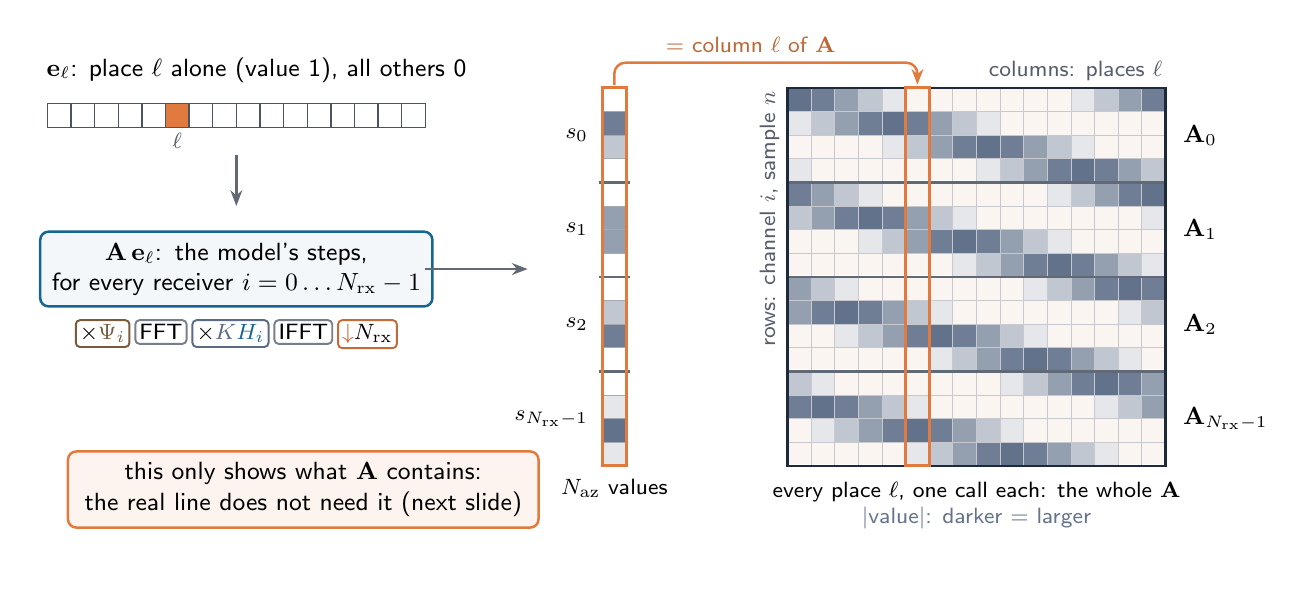
\begin{tikzpicture}[x=1cm,y=1cm,font=\footnotesize,
      ar/.style={-{Stealth[length=2.0mm]},line width=0.9pt,draw=ink!70},
      ix/.style={font=\footnotesize,text=ink!75,inner sep=1pt},
      chip/.style={rounded corners=1.5pt,line width=0.7pt,fill=white,inner sep=1.5pt,font=\footnotesize}]
    \path (-0.2,-1.0) rectangle (15.3,6.1);
    \def\cs{0.3}\def\xh{9.45}\def\yh{5.35}\def\L{5}\def\xs{7.1}
    % ---------------- the grid of A (empty), its blocks and axes
    \foreach \b in {0,...,3} \fill[fD!7] (\xh,{\yh-4*\b*\cs}) rectangle ({\xh+16*\cs},{\yh-(4*\b+4)*\cs+0.03});
    \foreach \c in {1,...,15} {\draw[ink!25,line width=0.3pt] ({\xh+\c*\cs},\yh) -- ({\xh+\c*\cs},{\yh-16*\cs}); \draw[ink!25,line width=0.3pt] (\xh,{\yh-\c*\cs}) -- ({\xh+16*\cs},{\yh-\c*\cs});}
    \foreach \b in {1,2,3} \draw[ink!70,line width=0.8pt] (\xh,{\yh-4*\b*\cs}) -- ({\xh+16*\cs},{\yh-4*\b*\cs});
    \draw[ink,line width=0.9pt] (\xh,\yh) rectangle ({\xh+16*\cs},{\yh-16*\cs});
    \foreach \b/\n in {0/{$\mathbf A_0$},1/{$\mathbf A_1$},2/{$\mathbf A_2$},3/{$\mathbf A_{N_{\mathrm{rx}}-1}$}}
      \node[anchor=west,font=\small] at ({\xh+16*\cs+0.1},{\yh-(4*\b+2)*\cs}) {\n};
    \node[anchor=south east,ix] at ({\xh+16*\cs},\yh+0.05) {columns: places $\ell$};
    \node[ix,rotate=90,anchor=south east] at (\xh-0.06,\yh) {rows: channel $i$, sample $n$};
    % ================= step 1: one place alone -> the model -> one column
    % the impulse e_l
    \node[anchor=south west,font=\small,inner sep=1pt] at (0.0,5.38) {$\mathbf e_\ell$: place $\ell$ alone (value 1), all others 0};
    \foreach \c in {0,...,15} \draw[fG!80,line width=0.5pt,fill=white] ({0.05+\c*\cs},4.85) rectangle ({0.05+(\c+1)*\cs},5.15);
    \fill[amber] ({0.05+\L*\cs},4.85) rectangle ({0.05+(\L+1)*\cs},5.15);
    \draw[fG!80,line width=0.5pt] ({0.05+\L*\cs},4.85) rectangle ({0.05+(\L+1)*\cs},5.15);
    \node[ix,anchor=north] at ({0.05+(\L+0.5)*\cs},4.82) {$\ell$};
    \draw[ar] (2.45,4.5) -- (2.45,3.85);
    % the model, as a function
    \node[rounded corners=3pt,draw=primary,line width=0.9pt,fill=primary!5,align=center,inner sep=4pt,font=\small,text width=4.7cm]
      (fw) at (2.45,3.05) {$\mathbf A\,\mathbf e_\ell$: the model's steps,\\ for every receiver $i=0\ldots N_{\mathrm{rx}}-1$};
    \node[anchor=north,inner sep=0pt] at (2.45,2.42) {%
      \tikz[baseline]{\node[chip,draw=fP]{$\times\fP$}; }\,\tikz[baseline]{\node[chip,draw=ink!60]{FFT};}\,%
      \tikz[baseline]{\node[chip,draw=fK]{$\times\fK\fH$};}\,\tikz[baseline]{\node[chip,draw=ink!60]{IFFT};}\,%
      \tikz[baseline]{\node[chip,draw=fD]{${\color{fD}\downarrow}N_{\mathrm{rx}}$};}};
    \draw[ar] (4.85,3.05) -- (\xs-0.95,3.05);
    % the output: one column, split into the N_rx channels
    \begin{scope}[shift={(\xs-\L*\cs,\yh)},scale=\cs]
      \clip (\L,0) rectangle (\L+1,-16);
      % generated by scripts/plot_v29.py: |A| of the toy, column l = LineModel.forward(e_l)
\fill[fK!95] (0,0) rectangle ++(1,-1);
\fill[fK!87] (1,0) rectangle ++(1,-1);
\fill[fK!65] (2,0) rectangle ++(1,-1);
\fill[fK!38] (3,0) rectangle ++(1,-1);
\fill[fK!16] (4,0) rectangle ++(1,-1);
\fill[fK!16] (12,0) rectangle ++(1,-1);
\fill[fK!38] (13,0) rectangle ++(1,-1);
\fill[fK!65] (14,0) rectangle ++(1,-1);
\fill[fK!87] (15,0) rectangle ++(1,-1);
\fill[fK!16] (0,-1) rectangle ++(1,-1);
\fill[fK!38] (1,-1) rectangle ++(1,-1);
\fill[fK!65] (2,-1) rectangle ++(1,-1);
\fill[fK!87] (3,-1) rectangle ++(1,-1);
\fill[fK!95] (4,-1) rectangle ++(1,-1);
\fill[fK!87] (5,-1) rectangle ++(1,-1);
\fill[fK!65] (6,-1) rectangle ++(1,-1);
\fill[fK!38] (7,-1) rectangle ++(1,-1);
\fill[fK!16] (8,-1) rectangle ++(1,-1);
\fill[fK!16] (4,-2) rectangle ++(1,-1);
\fill[fK!38] (5,-2) rectangle ++(1,-1);
\fill[fK!65] (6,-2) rectangle ++(1,-1);
\fill[fK!87] (7,-2) rectangle ++(1,-1);
\fill[fK!95] (8,-2) rectangle ++(1,-1);
\fill[fK!87] (9,-2) rectangle ++(1,-1);
\fill[fK!65] (10,-2) rectangle ++(1,-1);
\fill[fK!38] (11,-2) rectangle ++(1,-1);
\fill[fK!16] (12,-2) rectangle ++(1,-1);
\fill[fK!16] (0,-3) rectangle ++(1,-1);
\fill[fK!16] (8,-3) rectangle ++(1,-1);
\fill[fK!38] (9,-3) rectangle ++(1,-1);
\fill[fK!65] (10,-3) rectangle ++(1,-1);
\fill[fK!87] (11,-3) rectangle ++(1,-1);
\fill[fK!95] (12,-3) rectangle ++(1,-1);
\fill[fK!87] (13,-3) rectangle ++(1,-1);
\fill[fK!65] (14,-3) rectangle ++(1,-1);
\fill[fK!38] (15,-3) rectangle ++(1,-1);
\fill[fK!87] (0,-4) rectangle ++(1,-1);
\fill[fK!65] (1,-4) rectangle ++(1,-1);
\fill[fK!38] (2,-4) rectangle ++(1,-1);
\fill[fK!16] (3,-4) rectangle ++(1,-1);
\fill[fK!16] (11,-4) rectangle ++(1,-1);
\fill[fK!38] (12,-4) rectangle ++(1,-1);
\fill[fK!65] (13,-4) rectangle ++(1,-1);
\fill[fK!87] (14,-4) rectangle ++(1,-1);
\fill[fK!95] (15,-4) rectangle ++(1,-1);
\fill[fK!38] (0,-5) rectangle ++(1,-1);
\fill[fK!65] (1,-5) rectangle ++(1,-1);
\fill[fK!87] (2,-5) rectangle ++(1,-1);
\fill[fK!95] (3,-5) rectangle ++(1,-1);
\fill[fK!87] (4,-5) rectangle ++(1,-1);
\fill[fK!65] (5,-5) rectangle ++(1,-1);
\fill[fK!38] (6,-5) rectangle ++(1,-1);
\fill[fK!16] (7,-5) rectangle ++(1,-1);
\fill[fK!16] (15,-5) rectangle ++(1,-1);
\fill[fK!16] (3,-6) rectangle ++(1,-1);
\fill[fK!38] (4,-6) rectangle ++(1,-1);
\fill[fK!65] (5,-6) rectangle ++(1,-1);
\fill[fK!87] (6,-6) rectangle ++(1,-1);
\fill[fK!95] (7,-6) rectangle ++(1,-1);
\fill[fK!87] (8,-6) rectangle ++(1,-1);
\fill[fK!65] (9,-6) rectangle ++(1,-1);
\fill[fK!38] (10,-6) rectangle ++(1,-1);
\fill[fK!16] (11,-6) rectangle ++(1,-1);
\fill[fK!16] (7,-7) rectangle ++(1,-1);
\fill[fK!38] (8,-7) rectangle ++(1,-1);
\fill[fK!65] (9,-7) rectangle ++(1,-1);
\fill[fK!87] (10,-7) rectangle ++(1,-1);
\fill[fK!95] (11,-7) rectangle ++(1,-1);
\fill[fK!87] (12,-7) rectangle ++(1,-1);
\fill[fK!65] (13,-7) rectangle ++(1,-1);
\fill[fK!38] (14,-7) rectangle ++(1,-1);
\fill[fK!16] (15,-7) rectangle ++(1,-1);
\fill[fK!65] (0,-8) rectangle ++(1,-1);
\fill[fK!38] (1,-8) rectangle ++(1,-1);
\fill[fK!16] (2,-8) rectangle ++(1,-1);
\fill[fK!16] (10,-8) rectangle ++(1,-1);
\fill[fK!38] (11,-8) rectangle ++(1,-1);
\fill[fK!65] (12,-8) rectangle ++(1,-1);
\fill[fK!87] (13,-8) rectangle ++(1,-1);
\fill[fK!95] (14,-8) rectangle ++(1,-1);
\fill[fK!87] (15,-8) rectangle ++(1,-1);
\fill[fK!65] (0,-9) rectangle ++(1,-1);
\fill[fK!87] (1,-9) rectangle ++(1,-1);
\fill[fK!95] (2,-9) rectangle ++(1,-1);
\fill[fK!87] (3,-9) rectangle ++(1,-1);
\fill[fK!65] (4,-9) rectangle ++(1,-1);
\fill[fK!38] (5,-9) rectangle ++(1,-1);
\fill[fK!16] (6,-9) rectangle ++(1,-1);
\fill[fK!16] (14,-9) rectangle ++(1,-1);
\fill[fK!38] (15,-9) rectangle ++(1,-1);
\fill[fK!16] (2,-10) rectangle ++(1,-1);
\fill[fK!38] (3,-10) rectangle ++(1,-1);
\fill[fK!65] (4,-10) rectangle ++(1,-1);
\fill[fK!87] (5,-10) rectangle ++(1,-1);
\fill[fK!95] (6,-10) rectangle ++(1,-1);
\fill[fK!87] (7,-10) rectangle ++(1,-1);
\fill[fK!65] (8,-10) rectangle ++(1,-1);
\fill[fK!38] (9,-10) rectangle ++(1,-1);
\fill[fK!16] (10,-10) rectangle ++(1,-1);
\fill[fK!16] (6,-11) rectangle ++(1,-1);
\fill[fK!38] (7,-11) rectangle ++(1,-1);
\fill[fK!65] (8,-11) rectangle ++(1,-1);
\fill[fK!87] (9,-11) rectangle ++(1,-1);
\fill[fK!95] (10,-11) rectangle ++(1,-1);
\fill[fK!87] (11,-11) rectangle ++(1,-1);
\fill[fK!65] (12,-11) rectangle ++(1,-1);
\fill[fK!38] (13,-11) rectangle ++(1,-1);
\fill[fK!16] (14,-11) rectangle ++(1,-1);
\fill[fK!38] (0,-12) rectangle ++(1,-1);
\fill[fK!16] (1,-12) rectangle ++(1,-1);
\fill[fK!16] (9,-12) rectangle ++(1,-1);
\fill[fK!38] (10,-12) rectangle ++(1,-1);
\fill[fK!65] (11,-12) rectangle ++(1,-1);
\fill[fK!87] (12,-12) rectangle ++(1,-1);
\fill[fK!95] (13,-12) rectangle ++(1,-1);
\fill[fK!87] (14,-12) rectangle ++(1,-1);
\fill[fK!65] (15,-12) rectangle ++(1,-1);
\fill[fK!87] (0,-13) rectangle ++(1,-1);
\fill[fK!95] (1,-13) rectangle ++(1,-1);
\fill[fK!87] (2,-13) rectangle ++(1,-1);
\fill[fK!65] (3,-13) rectangle ++(1,-1);
\fill[fK!38] (4,-13) rectangle ++(1,-1);
\fill[fK!16] (5,-13) rectangle ++(1,-1);
\fill[fK!16] (13,-13) rectangle ++(1,-1);
\fill[fK!38] (14,-13) rectangle ++(1,-1);
\fill[fK!65] (15,-13) rectangle ++(1,-1);
\fill[fK!16] (1,-14) rectangle ++(1,-1);
\fill[fK!38] (2,-14) rectangle ++(1,-1);
\fill[fK!65] (3,-14) rectangle ++(1,-1);
\fill[fK!87] (4,-14) rectangle ++(1,-1);
\fill[fK!95] (5,-14) rectangle ++(1,-1);
\fill[fK!87] (6,-14) rectangle ++(1,-1);
\fill[fK!65] (7,-14) rectangle ++(1,-1);
\fill[fK!38] (8,-14) rectangle ++(1,-1);
\fill[fK!16] (9,-14) rectangle ++(1,-1);
\fill[fK!16] (5,-15) rectangle ++(1,-1);
\fill[fK!38] (6,-15) rectangle ++(1,-1);
\fill[fK!65] (7,-15) rectangle ++(1,-1);
\fill[fK!87] (8,-15) rectangle ++(1,-1);
\fill[fK!95] (9,-15) rectangle ++(1,-1);
\fill[fK!87] (10,-15) rectangle ++(1,-1);
\fill[fK!65] (11,-15) rectangle ++(1,-1);
\fill[fK!38] (12,-15) rectangle ++(1,-1);
\fill[fK!16] (13,-15) rectangle ++(1,-1);

    \end{scope}
    \foreach \c in {1,...,15} \draw[ink!40,line width=0.3pt] (\xs,{\yh-\c*\cs}) -- ({\xs+\cs},{\yh-\c*\cs});
    \foreach \b in {1,2,3} \draw[ink!70,line width=0.8pt] (\xs-0.05,{\yh-4*\b*\cs}) -- ({\xs+\cs+0.05},{\yh-4*\b*\cs});
    \draw[amber,line width=1.1pt] (\xs,\yh) rectangle ({\xs+\cs},{\yh-16*\cs});
    \foreach \b/\n in {0/s_0,1/s_1,2/s_2,3/{s_{N_{\mathrm{rx}}-1}}}
      \node[anchor=east,font=\footnotesize] at (\xs-0.06,{\yh-(4*\b+2)*\cs}) {$\n$};
    \node[anchor=north,font=\footnotesize,align=center] at ({\xs+0.15},{\yh-16*\cs-0.05}) {$N_{\mathrm{az}}$ values};
    \draw[ar,draw=amber,rounded corners=4pt] ({\xs+0.5*\cs},\yh+0.04) -- ({\xs+0.5*\cs},\yh+0.32)
      -- node[above,font=\footnotesize,text=amber!85!black,pos=0.45]{= column $\ell$ of $\mathbf A$} ({\xh+(\L+0.5)*\cs},\yh+0.32) -- ({\xh+(\L+0.5)*\cs},\yh+0.04);
    \begin{scope}[shift={(\xh,\yh)},scale=\cs]
      \clip (\L,0) rectangle (\L+1,-16);
      % generated by scripts/plot_v29.py: |A| of the toy, column l = LineModel.forward(e_l)
\fill[fK!95] (0,0) rectangle ++(1,-1);
\fill[fK!87] (1,0) rectangle ++(1,-1);
\fill[fK!65] (2,0) rectangle ++(1,-1);
\fill[fK!38] (3,0) rectangle ++(1,-1);
\fill[fK!16] (4,0) rectangle ++(1,-1);
\fill[fK!16] (12,0) rectangle ++(1,-1);
\fill[fK!38] (13,0) rectangle ++(1,-1);
\fill[fK!65] (14,0) rectangle ++(1,-1);
\fill[fK!87] (15,0) rectangle ++(1,-1);
\fill[fK!16] (0,-1) rectangle ++(1,-1);
\fill[fK!38] (1,-1) rectangle ++(1,-1);
\fill[fK!65] (2,-1) rectangle ++(1,-1);
\fill[fK!87] (3,-1) rectangle ++(1,-1);
\fill[fK!95] (4,-1) rectangle ++(1,-1);
\fill[fK!87] (5,-1) rectangle ++(1,-1);
\fill[fK!65] (6,-1) rectangle ++(1,-1);
\fill[fK!38] (7,-1) rectangle ++(1,-1);
\fill[fK!16] (8,-1) rectangle ++(1,-1);
\fill[fK!16] (4,-2) rectangle ++(1,-1);
\fill[fK!38] (5,-2) rectangle ++(1,-1);
\fill[fK!65] (6,-2) rectangle ++(1,-1);
\fill[fK!87] (7,-2) rectangle ++(1,-1);
\fill[fK!95] (8,-2) rectangle ++(1,-1);
\fill[fK!87] (9,-2) rectangle ++(1,-1);
\fill[fK!65] (10,-2) rectangle ++(1,-1);
\fill[fK!38] (11,-2) rectangle ++(1,-1);
\fill[fK!16] (12,-2) rectangle ++(1,-1);
\fill[fK!16] (0,-3) rectangle ++(1,-1);
\fill[fK!16] (8,-3) rectangle ++(1,-1);
\fill[fK!38] (9,-3) rectangle ++(1,-1);
\fill[fK!65] (10,-3) rectangle ++(1,-1);
\fill[fK!87] (11,-3) rectangle ++(1,-1);
\fill[fK!95] (12,-3) rectangle ++(1,-1);
\fill[fK!87] (13,-3) rectangle ++(1,-1);
\fill[fK!65] (14,-3) rectangle ++(1,-1);
\fill[fK!38] (15,-3) rectangle ++(1,-1);
\fill[fK!87] (0,-4) rectangle ++(1,-1);
\fill[fK!65] (1,-4) rectangle ++(1,-1);
\fill[fK!38] (2,-4) rectangle ++(1,-1);
\fill[fK!16] (3,-4) rectangle ++(1,-1);
\fill[fK!16] (11,-4) rectangle ++(1,-1);
\fill[fK!38] (12,-4) rectangle ++(1,-1);
\fill[fK!65] (13,-4) rectangle ++(1,-1);
\fill[fK!87] (14,-4) rectangle ++(1,-1);
\fill[fK!95] (15,-4) rectangle ++(1,-1);
\fill[fK!38] (0,-5) rectangle ++(1,-1);
\fill[fK!65] (1,-5) rectangle ++(1,-1);
\fill[fK!87] (2,-5) rectangle ++(1,-1);
\fill[fK!95] (3,-5) rectangle ++(1,-1);
\fill[fK!87] (4,-5) rectangle ++(1,-1);
\fill[fK!65] (5,-5) rectangle ++(1,-1);
\fill[fK!38] (6,-5) rectangle ++(1,-1);
\fill[fK!16] (7,-5) rectangle ++(1,-1);
\fill[fK!16] (15,-5) rectangle ++(1,-1);
\fill[fK!16] (3,-6) rectangle ++(1,-1);
\fill[fK!38] (4,-6) rectangle ++(1,-1);
\fill[fK!65] (5,-6) rectangle ++(1,-1);
\fill[fK!87] (6,-6) rectangle ++(1,-1);
\fill[fK!95] (7,-6) rectangle ++(1,-1);
\fill[fK!87] (8,-6) rectangle ++(1,-1);
\fill[fK!65] (9,-6) rectangle ++(1,-1);
\fill[fK!38] (10,-6) rectangle ++(1,-1);
\fill[fK!16] (11,-6) rectangle ++(1,-1);
\fill[fK!16] (7,-7) rectangle ++(1,-1);
\fill[fK!38] (8,-7) rectangle ++(1,-1);
\fill[fK!65] (9,-7) rectangle ++(1,-1);
\fill[fK!87] (10,-7) rectangle ++(1,-1);
\fill[fK!95] (11,-7) rectangle ++(1,-1);
\fill[fK!87] (12,-7) rectangle ++(1,-1);
\fill[fK!65] (13,-7) rectangle ++(1,-1);
\fill[fK!38] (14,-7) rectangle ++(1,-1);
\fill[fK!16] (15,-7) rectangle ++(1,-1);
\fill[fK!65] (0,-8) rectangle ++(1,-1);
\fill[fK!38] (1,-8) rectangle ++(1,-1);
\fill[fK!16] (2,-8) rectangle ++(1,-1);
\fill[fK!16] (10,-8) rectangle ++(1,-1);
\fill[fK!38] (11,-8) rectangle ++(1,-1);
\fill[fK!65] (12,-8) rectangle ++(1,-1);
\fill[fK!87] (13,-8) rectangle ++(1,-1);
\fill[fK!95] (14,-8) rectangle ++(1,-1);
\fill[fK!87] (15,-8) rectangle ++(1,-1);
\fill[fK!65] (0,-9) rectangle ++(1,-1);
\fill[fK!87] (1,-9) rectangle ++(1,-1);
\fill[fK!95] (2,-9) rectangle ++(1,-1);
\fill[fK!87] (3,-9) rectangle ++(1,-1);
\fill[fK!65] (4,-9) rectangle ++(1,-1);
\fill[fK!38] (5,-9) rectangle ++(1,-1);
\fill[fK!16] (6,-9) rectangle ++(1,-1);
\fill[fK!16] (14,-9) rectangle ++(1,-1);
\fill[fK!38] (15,-9) rectangle ++(1,-1);
\fill[fK!16] (2,-10) rectangle ++(1,-1);
\fill[fK!38] (3,-10) rectangle ++(1,-1);
\fill[fK!65] (4,-10) rectangle ++(1,-1);
\fill[fK!87] (5,-10) rectangle ++(1,-1);
\fill[fK!95] (6,-10) rectangle ++(1,-1);
\fill[fK!87] (7,-10) rectangle ++(1,-1);
\fill[fK!65] (8,-10) rectangle ++(1,-1);
\fill[fK!38] (9,-10) rectangle ++(1,-1);
\fill[fK!16] (10,-10) rectangle ++(1,-1);
\fill[fK!16] (6,-11) rectangle ++(1,-1);
\fill[fK!38] (7,-11) rectangle ++(1,-1);
\fill[fK!65] (8,-11) rectangle ++(1,-1);
\fill[fK!87] (9,-11) rectangle ++(1,-1);
\fill[fK!95] (10,-11) rectangle ++(1,-1);
\fill[fK!87] (11,-11) rectangle ++(1,-1);
\fill[fK!65] (12,-11) rectangle ++(1,-1);
\fill[fK!38] (13,-11) rectangle ++(1,-1);
\fill[fK!16] (14,-11) rectangle ++(1,-1);
\fill[fK!38] (0,-12) rectangle ++(1,-1);
\fill[fK!16] (1,-12) rectangle ++(1,-1);
\fill[fK!16] (9,-12) rectangle ++(1,-1);
\fill[fK!38] (10,-12) rectangle ++(1,-1);
\fill[fK!65] (11,-12) rectangle ++(1,-1);
\fill[fK!87] (12,-12) rectangle ++(1,-1);
\fill[fK!95] (13,-12) rectangle ++(1,-1);
\fill[fK!87] (14,-12) rectangle ++(1,-1);
\fill[fK!65] (15,-12) rectangle ++(1,-1);
\fill[fK!87] (0,-13) rectangle ++(1,-1);
\fill[fK!95] (1,-13) rectangle ++(1,-1);
\fill[fK!87] (2,-13) rectangle ++(1,-1);
\fill[fK!65] (3,-13) rectangle ++(1,-1);
\fill[fK!38] (4,-13) rectangle ++(1,-1);
\fill[fK!16] (5,-13) rectangle ++(1,-1);
\fill[fK!16] (13,-13) rectangle ++(1,-1);
\fill[fK!38] (14,-13) rectangle ++(1,-1);
\fill[fK!65] (15,-13) rectangle ++(1,-1);
\fill[fK!16] (1,-14) rectangle ++(1,-1);
\fill[fK!38] (2,-14) rectangle ++(1,-1);
\fill[fK!65] (3,-14) rectangle ++(1,-1);
\fill[fK!87] (4,-14) rectangle ++(1,-1);
\fill[fK!95] (5,-14) rectangle ++(1,-1);
\fill[fK!87] (6,-14) rectangle ++(1,-1);
\fill[fK!65] (7,-14) rectangle ++(1,-1);
\fill[fK!38] (8,-14) rectangle ++(1,-1);
\fill[fK!16] (9,-14) rectangle ++(1,-1);
\fill[fK!16] (5,-15) rectangle ++(1,-1);
\fill[fK!38] (6,-15) rectangle ++(1,-1);
\fill[fK!65] (7,-15) rectangle ++(1,-1);
\fill[fK!87] (8,-15) rectangle ++(1,-1);
\fill[fK!95] (9,-15) rectangle ++(1,-1);
\fill[fK!87] (10,-15) rectangle ++(1,-1);
\fill[fK!65] (11,-15) rectangle ++(1,-1);
\fill[fK!38] (12,-15) rectangle ++(1,-1);
\fill[fK!16] (13,-15) rectangle ++(1,-1);

    \end{scope}
    \draw[amber,line width=1.1pt] ({\xh+\L*\cs},\yh) rectangle ({\xh+(\L+1)*\cs},{\yh-16*\cs});
    % ================= step 2: every place, one call each -> the whole A
    \begin{scope}[visible on=<2->]
      \begin{scope}[shift={(\xh,\yh)},scale=\cs]
        % generated by scripts/plot_v29.py: |A| of the toy, column l = LineModel.forward(e_l)
\fill[fK!95] (0,0) rectangle ++(1,-1);
\fill[fK!87] (1,0) rectangle ++(1,-1);
\fill[fK!65] (2,0) rectangle ++(1,-1);
\fill[fK!38] (3,0) rectangle ++(1,-1);
\fill[fK!16] (4,0) rectangle ++(1,-1);
\fill[fK!16] (12,0) rectangle ++(1,-1);
\fill[fK!38] (13,0) rectangle ++(1,-1);
\fill[fK!65] (14,0) rectangle ++(1,-1);
\fill[fK!87] (15,0) rectangle ++(1,-1);
\fill[fK!16] (0,-1) rectangle ++(1,-1);
\fill[fK!38] (1,-1) rectangle ++(1,-1);
\fill[fK!65] (2,-1) rectangle ++(1,-1);
\fill[fK!87] (3,-1) rectangle ++(1,-1);
\fill[fK!95] (4,-1) rectangle ++(1,-1);
\fill[fK!87] (5,-1) rectangle ++(1,-1);
\fill[fK!65] (6,-1) rectangle ++(1,-1);
\fill[fK!38] (7,-1) rectangle ++(1,-1);
\fill[fK!16] (8,-1) rectangle ++(1,-1);
\fill[fK!16] (4,-2) rectangle ++(1,-1);
\fill[fK!38] (5,-2) rectangle ++(1,-1);
\fill[fK!65] (6,-2) rectangle ++(1,-1);
\fill[fK!87] (7,-2) rectangle ++(1,-1);
\fill[fK!95] (8,-2) rectangle ++(1,-1);
\fill[fK!87] (9,-2) rectangle ++(1,-1);
\fill[fK!65] (10,-2) rectangle ++(1,-1);
\fill[fK!38] (11,-2) rectangle ++(1,-1);
\fill[fK!16] (12,-2) rectangle ++(1,-1);
\fill[fK!16] (0,-3) rectangle ++(1,-1);
\fill[fK!16] (8,-3) rectangle ++(1,-1);
\fill[fK!38] (9,-3) rectangle ++(1,-1);
\fill[fK!65] (10,-3) rectangle ++(1,-1);
\fill[fK!87] (11,-3) rectangle ++(1,-1);
\fill[fK!95] (12,-3) rectangle ++(1,-1);
\fill[fK!87] (13,-3) rectangle ++(1,-1);
\fill[fK!65] (14,-3) rectangle ++(1,-1);
\fill[fK!38] (15,-3) rectangle ++(1,-1);
\fill[fK!87] (0,-4) rectangle ++(1,-1);
\fill[fK!65] (1,-4) rectangle ++(1,-1);
\fill[fK!38] (2,-4) rectangle ++(1,-1);
\fill[fK!16] (3,-4) rectangle ++(1,-1);
\fill[fK!16] (11,-4) rectangle ++(1,-1);
\fill[fK!38] (12,-4) rectangle ++(1,-1);
\fill[fK!65] (13,-4) rectangle ++(1,-1);
\fill[fK!87] (14,-4) rectangle ++(1,-1);
\fill[fK!95] (15,-4) rectangle ++(1,-1);
\fill[fK!38] (0,-5) rectangle ++(1,-1);
\fill[fK!65] (1,-5) rectangle ++(1,-1);
\fill[fK!87] (2,-5) rectangle ++(1,-1);
\fill[fK!95] (3,-5) rectangle ++(1,-1);
\fill[fK!87] (4,-5) rectangle ++(1,-1);
\fill[fK!65] (5,-5) rectangle ++(1,-1);
\fill[fK!38] (6,-5) rectangle ++(1,-1);
\fill[fK!16] (7,-5) rectangle ++(1,-1);
\fill[fK!16] (15,-5) rectangle ++(1,-1);
\fill[fK!16] (3,-6) rectangle ++(1,-1);
\fill[fK!38] (4,-6) rectangle ++(1,-1);
\fill[fK!65] (5,-6) rectangle ++(1,-1);
\fill[fK!87] (6,-6) rectangle ++(1,-1);
\fill[fK!95] (7,-6) rectangle ++(1,-1);
\fill[fK!87] (8,-6) rectangle ++(1,-1);
\fill[fK!65] (9,-6) rectangle ++(1,-1);
\fill[fK!38] (10,-6) rectangle ++(1,-1);
\fill[fK!16] (11,-6) rectangle ++(1,-1);
\fill[fK!16] (7,-7) rectangle ++(1,-1);
\fill[fK!38] (8,-7) rectangle ++(1,-1);
\fill[fK!65] (9,-7) rectangle ++(1,-1);
\fill[fK!87] (10,-7) rectangle ++(1,-1);
\fill[fK!95] (11,-7) rectangle ++(1,-1);
\fill[fK!87] (12,-7) rectangle ++(1,-1);
\fill[fK!65] (13,-7) rectangle ++(1,-1);
\fill[fK!38] (14,-7) rectangle ++(1,-1);
\fill[fK!16] (15,-7) rectangle ++(1,-1);
\fill[fK!65] (0,-8) rectangle ++(1,-1);
\fill[fK!38] (1,-8) rectangle ++(1,-1);
\fill[fK!16] (2,-8) rectangle ++(1,-1);
\fill[fK!16] (10,-8) rectangle ++(1,-1);
\fill[fK!38] (11,-8) rectangle ++(1,-1);
\fill[fK!65] (12,-8) rectangle ++(1,-1);
\fill[fK!87] (13,-8) rectangle ++(1,-1);
\fill[fK!95] (14,-8) rectangle ++(1,-1);
\fill[fK!87] (15,-8) rectangle ++(1,-1);
\fill[fK!65] (0,-9) rectangle ++(1,-1);
\fill[fK!87] (1,-9) rectangle ++(1,-1);
\fill[fK!95] (2,-9) rectangle ++(1,-1);
\fill[fK!87] (3,-9) rectangle ++(1,-1);
\fill[fK!65] (4,-9) rectangle ++(1,-1);
\fill[fK!38] (5,-9) rectangle ++(1,-1);
\fill[fK!16] (6,-9) rectangle ++(1,-1);
\fill[fK!16] (14,-9) rectangle ++(1,-1);
\fill[fK!38] (15,-9) rectangle ++(1,-1);
\fill[fK!16] (2,-10) rectangle ++(1,-1);
\fill[fK!38] (3,-10) rectangle ++(1,-1);
\fill[fK!65] (4,-10) rectangle ++(1,-1);
\fill[fK!87] (5,-10) rectangle ++(1,-1);
\fill[fK!95] (6,-10) rectangle ++(1,-1);
\fill[fK!87] (7,-10) rectangle ++(1,-1);
\fill[fK!65] (8,-10) rectangle ++(1,-1);
\fill[fK!38] (9,-10) rectangle ++(1,-1);
\fill[fK!16] (10,-10) rectangle ++(1,-1);
\fill[fK!16] (6,-11) rectangle ++(1,-1);
\fill[fK!38] (7,-11) rectangle ++(1,-1);
\fill[fK!65] (8,-11) rectangle ++(1,-1);
\fill[fK!87] (9,-11) rectangle ++(1,-1);
\fill[fK!95] (10,-11) rectangle ++(1,-1);
\fill[fK!87] (11,-11) rectangle ++(1,-1);
\fill[fK!65] (12,-11) rectangle ++(1,-1);
\fill[fK!38] (13,-11) rectangle ++(1,-1);
\fill[fK!16] (14,-11) rectangle ++(1,-1);
\fill[fK!38] (0,-12) rectangle ++(1,-1);
\fill[fK!16] (1,-12) rectangle ++(1,-1);
\fill[fK!16] (9,-12) rectangle ++(1,-1);
\fill[fK!38] (10,-12) rectangle ++(1,-1);
\fill[fK!65] (11,-12) rectangle ++(1,-1);
\fill[fK!87] (12,-12) rectangle ++(1,-1);
\fill[fK!95] (13,-12) rectangle ++(1,-1);
\fill[fK!87] (14,-12) rectangle ++(1,-1);
\fill[fK!65] (15,-12) rectangle ++(1,-1);
\fill[fK!87] (0,-13) rectangle ++(1,-1);
\fill[fK!95] (1,-13) rectangle ++(1,-1);
\fill[fK!87] (2,-13) rectangle ++(1,-1);
\fill[fK!65] (3,-13) rectangle ++(1,-1);
\fill[fK!38] (4,-13) rectangle ++(1,-1);
\fill[fK!16] (5,-13) rectangle ++(1,-1);
\fill[fK!16] (13,-13) rectangle ++(1,-1);
\fill[fK!38] (14,-13) rectangle ++(1,-1);
\fill[fK!65] (15,-13) rectangle ++(1,-1);
\fill[fK!16] (1,-14) rectangle ++(1,-1);
\fill[fK!38] (2,-14) rectangle ++(1,-1);
\fill[fK!65] (3,-14) rectangle ++(1,-1);
\fill[fK!87] (4,-14) rectangle ++(1,-1);
\fill[fK!95] (5,-14) rectangle ++(1,-1);
\fill[fK!87] (6,-14) rectangle ++(1,-1);
\fill[fK!65] (7,-14) rectangle ++(1,-1);
\fill[fK!38] (8,-14) rectangle ++(1,-1);
\fill[fK!16] (9,-14) rectangle ++(1,-1);
\fill[fK!16] (5,-15) rectangle ++(1,-1);
\fill[fK!38] (6,-15) rectangle ++(1,-1);
\fill[fK!65] (7,-15) rectangle ++(1,-1);
\fill[fK!87] (8,-15) rectangle ++(1,-1);
\fill[fK!95] (9,-15) rectangle ++(1,-1);
\fill[fK!87] (10,-15) rectangle ++(1,-1);
\fill[fK!65] (11,-15) rectangle ++(1,-1);
\fill[fK!38] (12,-15) rectangle ++(1,-1);
\fill[fK!16] (13,-15) rectangle ++(1,-1);

      \end{scope}
      \foreach \c in {1,...,15} {\draw[ink!25,line width=0.3pt] ({\xh+\c*\cs},\yh) -- ({\xh+\c*\cs},{\yh-16*\cs}); \draw[ink!25,line width=0.3pt] (\xh,{\yh-\c*\cs}) -- ({\xh+16*\cs},{\yh-\c*\cs});}
      \foreach \b in {1,2,3} \draw[ink!70,line width=0.8pt] (\xh,{\yh-4*\b*\cs}) -- ({\xh+16*\cs},{\yh-4*\b*\cs});
      \draw[ink,line width=0.9pt] (\xh,\yh) rectangle ({\xh+16*\cs},{\yh-16*\cs});
      \draw[amber,line width=1.1pt] ({\xh+\L*\cs},\yh) rectangle ({\xh+(\L+1)*\cs},{\yh-16*\cs});
      \node[anchor=north,font=\footnotesize,align=center] at ({\xh+8*\cs},{\yh-16*\cs-0.08})
        {every place $\ell$, one call each: the whole $\mathbf A$\\ {\color{muted}$|\text{value}|$: darker = larger}};
    \end{scope}
    % ================= step 3: the real line: never filled
    \begin{scope}[visible on=<3->]
      \node[rounded corners=3pt,draw=amber,line width=0.9pt,fill=amber!8,align=center,inner xsep=6pt,inner ysep=4pt,font=\small]
        at (3.3,0.25) {this only shows what $\mathbf A$ contains:\\ the real line does not need it (next slide)};
    \end{scope}
  \end{tikzpicture}
\end{document}
